\subsection{Evaluación y resultados}

Para validar la efectividad del proceso de especialización, se llevó a cabo una evaluación comparativa entre el modelo preentrenado y el modelo ajustado. Esta evaluación se centró en tres aspectos clave: fidelidad visual, coherencia semántica y adecuación morfológica a partir de un mismo prompt textual.

\subsubsection{Limitaciones del modelo base}

Aunque el modelo preentrenado Stable Diffusion v1.4 proporciona resultados visuales aceptables en muchos casos, se observaron importantes deficiencias al generar imágenes de conceptos específicos poco frecuentes, como ciertas razas de perros. Estas limitaciones afectan principalmente la coherencia anatómica y el realismo visual, lo que compromete su aplicabilidad en contextos especializados.

A modo de ejemplo, se utilizó el prompt:

\begin{center}
\textit{``a photo of a golden retriever''}
\end{center}

\subsubsection{Resultado con el modelo preentrenado}

La imagen generada por el modelo base presenta notables defectos: desalineación de los ojos, artefactos digitales en el hocico y una postura general poco natural. Aunque el color del pelaje podría sugerir la raza objetivo, la representación morfológica no es fiel ni reconocible.

\begin{figure}[H]
    \centering
    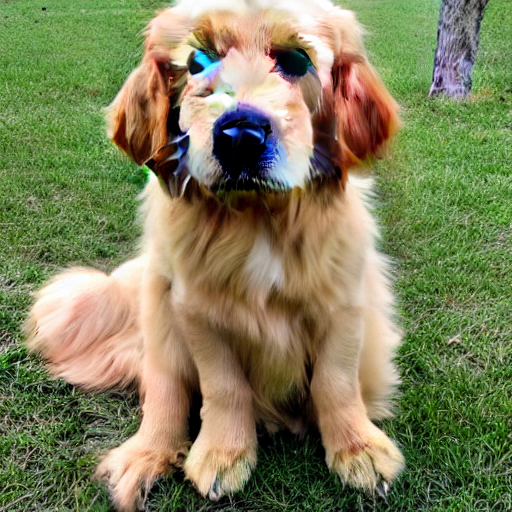
\includegraphics[width=0.45\textwidth]{golden_retriever_before.png}
    \caption{Resultado generado por el modelo preentrenado.}
    \label{fig:golden-before}
\end{figure}

\subsubsection{Resultado tras la especialización del modelo}

Tras aplicar la técnica de modificación del espacio latente, el modelo fue capaz de representar de forma mucho más precisa la raza solicitada. La imagen resultante muestra un perro con expresión realista, pelaje detallado, proporciones correctas y una pose reconocible. El resultado evidencia una mejora tanto estética como semántica.

\begin{figure}[H]
    \centering
    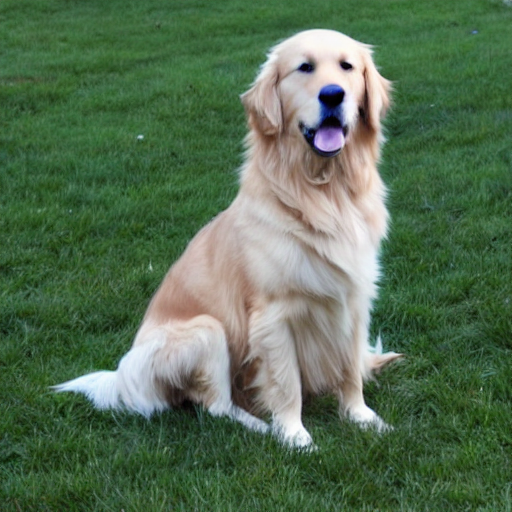
\includegraphics[width=0.45\textwidth]{golden_retriever_after.png}
    \caption{Resultado generado tras la especialización del modelo.}
    \label{fig:golden-after}
\end{figure}

\subsubsection{Evaluación de coherencia semántica con CLIP}

Para respaldar cuantitativamente esta mejora, se empleó el modelo \texttt{CLIP ViT-L/14}, que permite calcular la similitud entre imágenes y texto. Se utilizó el concepto de \textit{CLIP Score relativo}, que compara la afinidad de dos imágenes frente a un mismo prompt.

\begin{table}[H]
\centering
\renewcommand{\arraystretch}{1.5}
\begin{tabular}{|p{6cm}|c|}
\hline
\rowcolor{gray!30}
\textbf{Imagen generada} & \textbf{CLIP Score relativo} \\
\hline
Modelo preentrenado & 0.0659 \\
\hline
Modelo especializado & 0.9341 \\
\hline
\end{tabular}
\caption{Similitud relativa medida con CLIP}
\label{tab:clip-golden}
\end{table}

\begin{figure}[H]
    \centering
    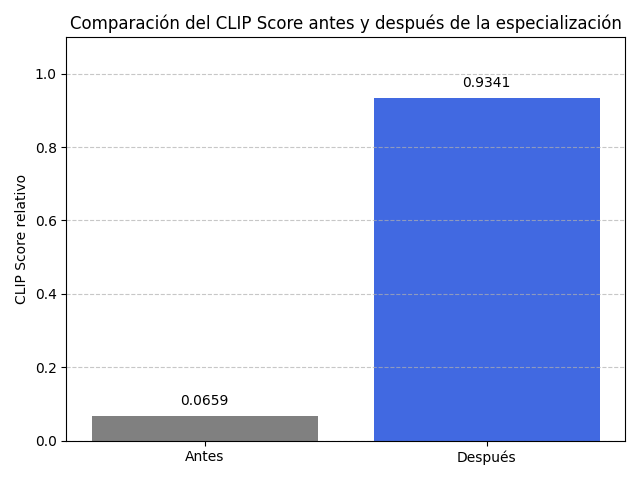
\includegraphics[width=0.45\textwidth]{clip-bar.png}
    \caption{Comparación visual del CLIP Score relativo.}
    \label{fig:clip-bar}
\end{figure}

\subsubsection{Síntesis de resultados}

La Figura~\ref{fig:clip-bar} visualiza de forma clara la mejora lograda. Mientras que el modelo original apenas logra asociar la imagen con el concepto de “golden retriever”, el modelo especializado alcanza un nivel de coherencia semántica casi perfecto. Esto confirma que la técnica utilizada no solo mejora la calidad visual, sino también la capacidad del modelo para representar correctamente conceptos específicos.

\subsubsection{Análisis del coste de entrenamiento}

Para evaluar la viabilidad del entrenamiento personalizado, se midieron los principales factores que impactan en el coste computacional del proceso. Estos valores permiten estimar la escalabilidad del enfoque en distintos entornos de ejecución.

\begin{table}[H]
\centering
\renewcommand{\arraystretch}{1.5}
\begin{tabular}{|p{5cm}|p{9cm}|}
\hline
\rowcolor{gray!30}
\textbf{Recurso} & \textbf{Especificaciones del servidor utilizado} \\
\hline
Procesador & AMD Ryzen Threadripper 2920X, 12 núcleos físicos, 24 hilos, hasta 3.5 GHz \\
\hline
Memoria RAM & 62 GiB totales, disponibles: 60 GiB libres \\
\hline
GPU & 2x NVIDIA TITAN RTX, 24 GiB de VRAM cada una \\
\hline
Sistema operativo & Ubuntu 24.04, kernel 6.8.0-59-generic, arquitectura x86\_64 \\
\hline
CUDA y Drivers & CUDA 12.4, Driver NVIDIA 550.163.01 \\
\hline
Duración del entrenamiento & Aprox. 5 horas \\
\hline
Tamaño del modelo entrenado & 4.0K (tamaño en disco del directorio \texttt{stable-dog-output}) \\
\hline
Frameworks utilizados & \texttt{diffusers}, \texttt{transformers}, \texttt{PyTorch}, \texttt{torchvision} \\
\hline
Técnicas aplicadas & DreamBooth, checkpointing, half precision (float16), batch size adaptativo \\
\hline
\end{tabular}
\caption{Recursos técnicos del servidor utilizado para el entrenamiento final}
\label{tab:servidor-entrenamiento}
\end{table}

\subsubsection{Evaluación de la generalización del modelo}

Además de mejorar la generación de razas específicas como el \textit{golden retriever}, resulta clave comprobar si el modelo especializado conserva su capacidad para generar imágenes no relacionadas con el entrenamiento. Para ello, se utilizó un prompt genérico:

\begin{center}
\textit{``a man sitting on a bench in a park''}
\end{center}

La generación se realizó antes y después de aplicar la especificación para evaluar posibles pérdidas de generalidad.

\paragraph{\textbf{Antes del entrenamiento especializado}} \mbox{}\\[0.5em]
El modelo preentrenado genera una escena coherente: un hombre de espaldas sentado en un banco, con árboles bien definidos y composición equilibrada. El resultado es visualmente aceptable y semánticamente correcto.

\begin{figure}[H]
    \centering
    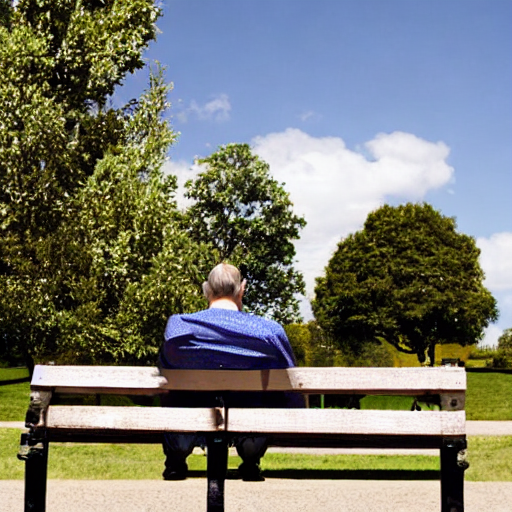
\includegraphics[width=0.45\textwidth]{man_before.png}
    \caption{Imagen generada por el modelo base con el prompt ``a man sitting on a bench in a park''.}
    \label{fig:man-before}
\end{figure}

\paragraph{\textbf{Después del entrenamiento especializado}} \mbox{}\\[0.5em]
Tras la especialización en razas de perro, el modelo mantiene su capacidad para representar correctamente conceptos no entrenados. La escena generada presenta un entorno similar, con árboles, banco y persona reconocibles, sin signos de sobreajuste. Esto sugiere que la adaptación ha sido localizada y no ha afectado negativamente a la generalización.

\begin{figure}[H]
    \centering
    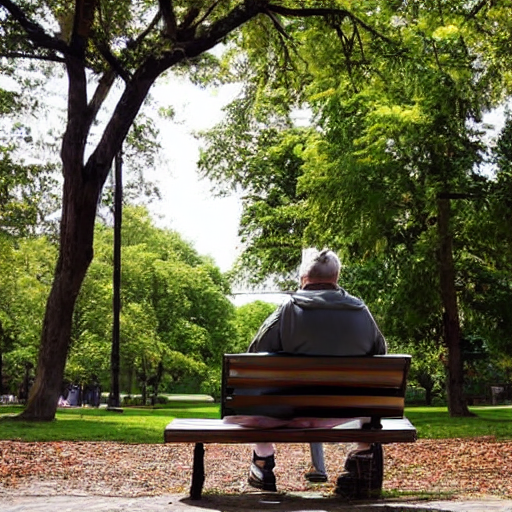
\includegraphics[width=0.45\textwidth]{man_after.png}
    \caption{Imagen generada por el modelo especializado con el mismo prompt.}
    \label{fig:man-after}
\end{figure}

\paragraph{\textbf{Conclusión}} \mbox{}\\[0.5em]
La comparación cualitativa sugiere que el modelo mantiene una buena capacidad de generalización tras la especialización. Es capaz de generar imágenes coherentes incluso para descripciones no incluidas en el entrenamiento, lo que refuerza la aplicabilidad del enfoque de DreamBooth en contextos donde es crucial preservar el conocimiento base del modelo.
